% ----------------------------------------
% Chap: Versuche auf dem EHD-Messgerät
% ----------------------------------------
\chapter{Versuche auf dem EHD-Messgerät}
\label{chap:versuche_auf_dem_ehd_messgeraet}

Um die Schmierfilmdicke im EHD-Komtakt mittels des elektrischen Verfahrens zu bestimmen, braucht man Kenntnis von den dielektrischen Eigenschaften des Schmierstoffes: deren Abhängigkeit von der Temperatur und dem Druck.

% ----------------------------------------
% Sec: Bestimmung der Dielektrizitätskonstante
% ----------------------------------------
\section{Dielektrizitätskonstante des Schmierstoffes}
\label{sec:dielektrizitaetskonstate_des_schmierstoffes}

Die Bestimmung der Dielektrizitätskonstante der Ölen \textit{FVA 3} und \textit{SHC320} wurde an einem kapazitiven Wegmessgerät durchgeführt.
Das Messgerät besteht aus zwei Stahlbacken, die auf einem Gestell aufgehängt werden, einem Zylinder und der elektronischen Einheit (siehe Abbildung~\ref{fig:das_kapazitive_wegmessgeraet}).

% ----------------------------------------
% Fig: Kapazitiv Wegmessgerät beim IMKT
% ----------------------------------------
\begin{figure}[htb]
    \centering
    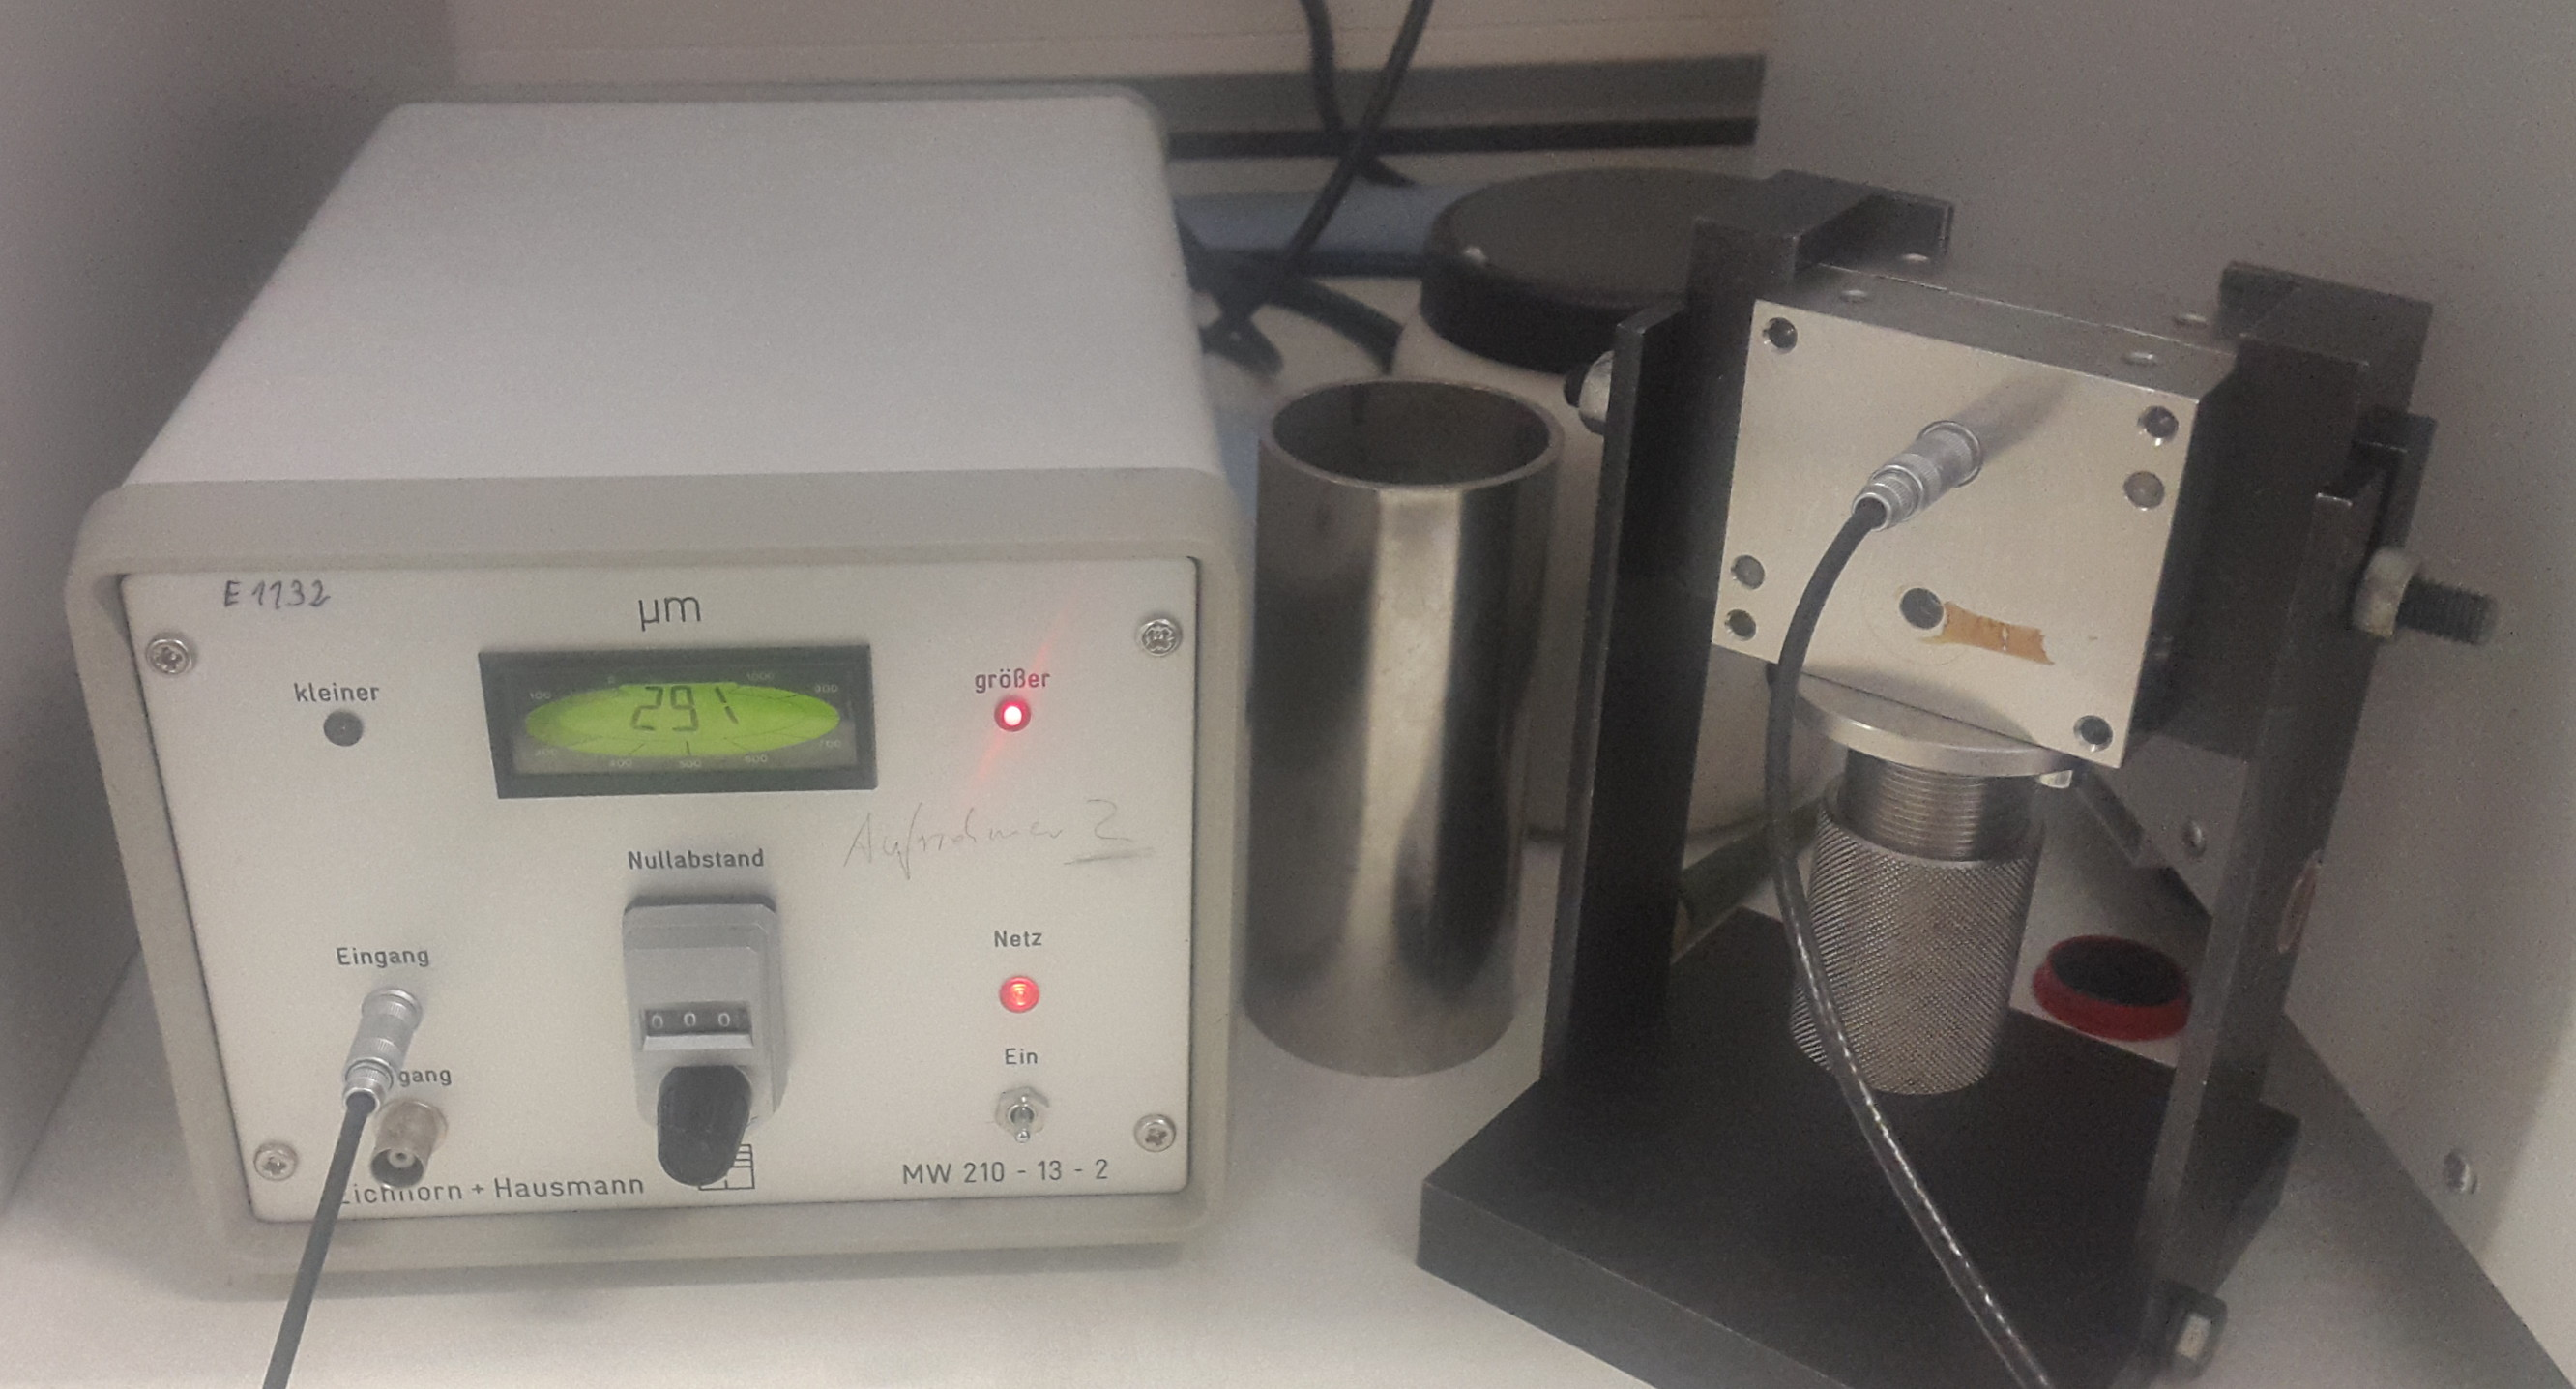
\includegraphics[]{./images/wegmessgeraet_imkt.pdf}
    \caption{Das kapazitive Wegmessgerät zur Bestimmung der Dielektrizitätskonstante des \textit{FVA 3} Öl}
    \label{fig:das_kapazitive_wegmessgeraet}
\end{figure}

Abbildung~\ref{fig:wegmessgeraet_pruefkopf} zeigt den Prüfkopf des Wegmessgeräts im abgebauten Zustand.
An einem Backen befindet sich der Wegsensor, welcher bündig mit der Innenseite des Backens sitzt.
Bei dem anderen Backen wurde eine Nut auf der inneren Oberfläche angebracht, sodass, wenn beide Backen zusammen verschraubt werden, sich dazwischen ein Spalt bildet.
Der Zylinder wird an der unteren Seite des Backens angeflanscht.
Durch das Drehen der Mutter wird der Kolben nach oben gedrückt, damit wird das Öl in den Spalt gepumpt.

% ----------------------------------------
% Fig: Funktionsprinzip des Prüfkopfs des Messgeräts
% ----------------------------------------
\begin{figure}[htb]
    \centering
    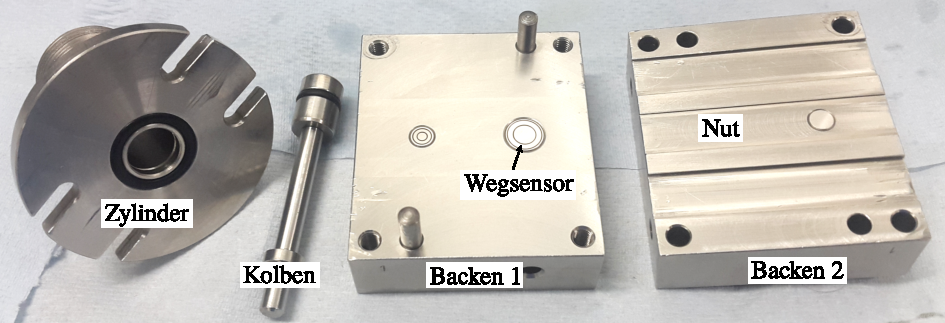
\includegraphics[]{./images/wegmessgeraet_pruefkopf.pdf}
    \caption{Der abgebaute Prüfkopf des Wegmessgeräts}
    \label{fig:wegmessgeraet_pruefkopf}
\end{figure}

Die Messung der Höhe des Spalts zwischen den Backen erfolgt durch dessen Betrachtung als Plattenkondensator, welcher die Luft als Dielektrikum hat (siehe Abbildung~\ref{fig:plattenkondensator}).
Beim Befördern des Öls in den Spalt ändert sich das Dielektrikum von Luft zu Luft + Öl, damit verändert sich seine Kapazität bzw. der Messwert, obwohl der Abstand im Spalt konstant bleibt.
Durch dieses Phänomen wird die Dielektrizitätskonstante des Öls als das Verhältnis zwischen den Messwegen bei Luft und beim Öl berechnet.
Die Messergebnisse für Öle \textit{FVA3} und \textit{SHC320} bei verschiedenen Temperaturen --- \SIrange{40}{80}{\degreeCelsius} --- werden in Tabelle~\ref{tab:relative_permittivitaet_fva3} dargestellt.

% ----------------------------------------
% Tab: Permittivität des FVA 3 Ols
% ----------------------------------------
\begin{minipage}[b]{0.55\linewidth}
    \centering
    \begin{tabular}{lrrr}
    Medium  & Temp [\si{\degreeCelsius}] & Weg [\si{\um}] & rel. Permittivität \\
    \hline
    Luft    & 20                         & 292            & 1                  \\
    FVA 3   & 40                         & 141            & 2.070              \\
    FVA 3   & 60                         & 142            & 2.056              \\
    FVA 3   & 80                         & 144            & 2.027              \\
    SHC 320 & 40                         & 118            & 2.474              \\
    SHC 320 & 60                         & 120            & 2.433              \\
    SHC 320 & 80                         & 122            & 2.393              \\
\end{tabular}

    \captionof{table}{relative Permittivität von Ölen bei unterschiedlichen Temperaturen}
    \label{tab:relative_permittivitaet_fva3}
\end{minipage}
\hspace{0.5cm}
%
% ----------------------------------------
% Fig: Plattenkondensator
% ----------------------------------------
\begin{minipage}[b]{0.3\linewidth}
    \centering
    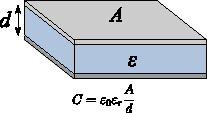
\includegraphics[width=\textwidth]{./images/plattenkondensator.pdf}
    \captionof{figure}{Plattenkondensator \cite{kondensator_wiki}}
    \label{fig:plattenkondensator}
\end{minipage}

% ----------------------------------------
% Sec: Kapazitive Messgeräte zur Schmierfilmdickenbestimmung
% ----------------------------------------
\section{Kapazitive Messgeräte zur Schmierfilmdickenbestimmung}
\label{sec:kapazitive_messgeraete_zur_schmierfilmdickenbestimmung}

% ----------------------------------------
% Sub: Stromladekurve Messgerät
% ----------------------------------------
\subsection{Stromladekurve Messgerät}
\label{sub:stromladekurve_messgeraet}

Im IMKT gibt es ein mobiles Messsystem zur Schmierfilmdickenmessung mittels kapazitiven Messverfahren.
Das System besteht aus einem Laptop, der mit \textit{Laderkurve-Software} installiert ist, und einer Messkarte (Typ USB-6211) von der Firma National Instrument (NI).
Bei der kapazitiven Messmethode wird der EHD-Kontakt als ein Kondensator $C_K$ betrachtet.
Die Aufladung des Kondensators erfolgt durch eine Ladespannung $U_L =$ \SI{0,2}{\volt} und einen Vorwiderstand $R_V =$ \SI{10}{\mega\ohm}.
Eine hohe Ladespannung ist unerwünscht, weil dieses zur Ionisierung des Schmierstoffes führt.
Das kann die Messergebnisse durch den Durchschlag des Kondensators verfälschen.
Mit dieser Konfiguration hat das Gerät eine höchste Auflösung von \SI{0.078}{\pico\farad} (siehe \ref{sec:aufloesung_des_mobilen_messsystems} im Anhang für die Berechnung).
Den schematischen Aufbau des mobilen Messsystems wird in Abbildung~\ref{fig:schematischer_aufbau_des_mobilen_messsystems} dargestellt.

% ----------------------------------------
% Fig: Schematischer Aufbau des mobilen Messsystems
% ----------------------------------------
\begin{figure}[htb]
    \centering
    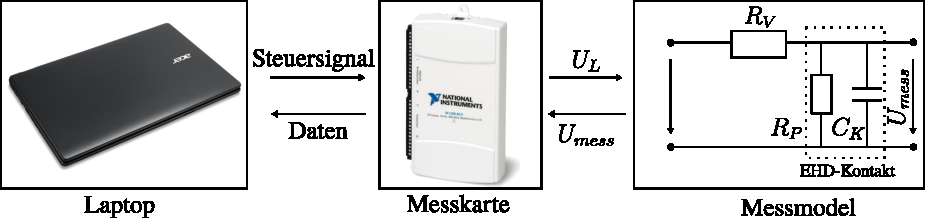
\includegraphics[]{./images/schematischer_aufbau_des_mobilen_messsystem.pdf}
    \caption{Schematischer Aufbau des mobilen Messsystems}
    \label{fig:schematischer_aufbau_des_mobilen_messsystems}
\end{figure}

Der Ladevorgang des Kondensators wird durch eine Zeitkonstante $\tau$ charakterisiert und in die Abbildung~\ref{fig:ladevorgang_eines_kondensators} dargestellt.
Zur Bestimmung der Zeitkonstante $\tau$ kann man durch die Anpassung der Ladekurve mit der Formel~\ref{eq:kondensator_e_funktion} oder im einen Zeitintervall $\Delta t$ zwischen den beiden definierten Spannungsgrenzen $U_1$ und $U_2$ (Formel~\ref{eq:bestimmung_der_zeitkonstante}) während des Ladevorgangs ermittelt.
Bei der Auswertung der Zeitkonstante mit der Formel~\ref{eg:kondensator_zeitkonstate} erhält man die Kapazität des EHD-Kontakts.

% ----------------------------------------
% Eq: Bestimmung der Zeitkonstante tau
% ----------------------------------------
\begin{minipage}[b]{0.3\textwidth}
    \begin{equation}
        U_C = U_L (1 - e ^ {-t/\tau})
        \label{eq:kondensator_e_funktion}
    \end{equation}
\end{minipage}
%
\begin{minipage}[b]{0.3\textwidth}
    \begin{equation}
        \tau = \cfrac{\Delta t}{\ln \cfrac{U_L - U_1}{U_L - U_2}}
        \label{eq:bestimmung_der_zeitkonstante}
    \end{equation}
\end{minipage}
%
\begin{minipage}[b]{0.3\textwidth}
    \begin{equation}
        C = \tau / R_V
        \label{eg:kondensator_zeitkonstate}
    \end{equation}
\end{minipage}

% ----------------------------------------
% Fig: Ladevorgang des Kondensators
% ----------------------------------------
\begin{figure}[htb]
    \centering
    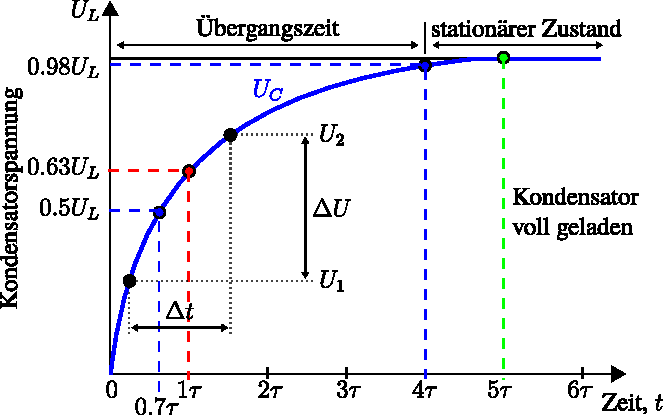
\includegraphics[]{./images/kondensator_ladevorgang.pdf}
    \caption{Der von Zeitkonstante $\tau$ charakterisierte Ladevorgang eines Kondensators}
    \label{fig:ladevorgang_eines_kondensators}
\end{figure}

Das ganze Messsystem wird von der \textit{Laderkurve-Software} gesteuert.
Sie misst nicht direkt die Kapazität, sondern sie nimmt die Antwort bzw. Ladekurve des ``Kondensators'' auf.
Die Auswertung für die Kapazität bzw. Filmdicke wird später mit einem Skript ausgeführt.
Die Software kann die Ladekurve in zwei Modi --- \emph{Anzahl der Messwerte} oder \emph{Messung nach Zeit} --- aufnehmen.
Im Rahmen dieser Arbeit werden alle Messungen mit dem ersten Modus durchgeführt.
Abbildung~\ref{fig:gui_der_laderkurve_software} zeigt die Benutzeroberfläche und die Einstellungen der Ladekurve-Software bei einer Testmessung mit einem Referenz-Kondensator (\SI{3.3}{\nano\farad}) an.

% ----------------------------------------
% Fig: GUI der Ladekurve-Software
% ----------------------------------------
\begin{figure}[htb]
    \centering
    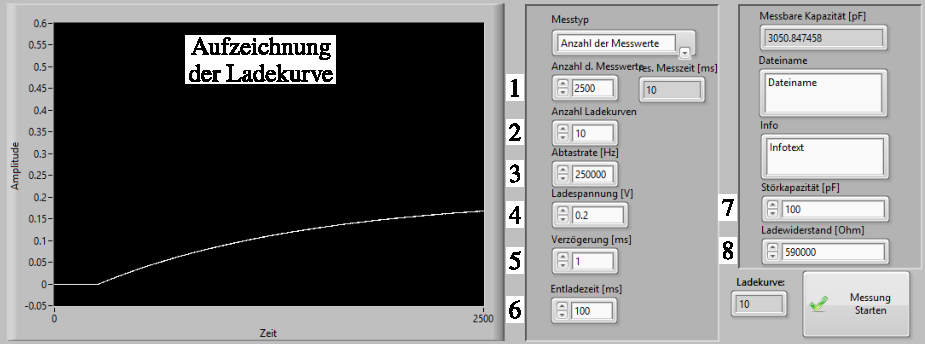
\includegraphics[]{./images/ladekurven_gui.pdf}
    \caption{Benutzeroberfläche der Laderkurve-Software}
    \label{fig:gui_der_laderkurve_software}
\end{figure}

Die Software ist relativ einfach zu bedienen, allerdings gibt es folgende Punkte, auf die man beachten muss:
% ----------------------------------------
% List: Optionen der Ladekurve Software
% ----------------------------------------
\begin{description}
    \item[1. Die Anzahl der Messwerte] ist die Auflösung der Messungen.
        Zu niedrige Werte können zu Messfehlern führen und zu hohe Werte kann es schnell den Speicher füllen.
        Der Standardwert ist \num{2500}.

    \item[2. Die Anzahl der Ladekurven] ist die Anzahl der Messungen, die nach einander durchgeführt werden.
        Der Standardwert ist \num{10}.

    \item[3. Die Abtastrate] ist die Anzahl der Messwerte, die die Messkarte pro Sekunde messen kann.
        Die USB-6211 Messkarte von NI kann maximal \SI[per-mode=symbol]{250}{\kilo\sample\per\second}, das entspricht \num{2500} Messwerte in einem Zeitraum von \SI{10}{\milli\second}, messen.

    \item[4. Die Ladespannung] ist die Spannung zwischen zwei Terminals des Kondensators.
        Der Wert sollte im Bereich von \SIrange{0.2}{0.5}{\volt} liegen.

    \item[5. Die Verzögerung] ist die Wartezeit, die die Software benötigt, bevor sie eine Messung ausführen kann.
        Der Standardwert ist \SI{1}{\ms}.

    \item[6. Die Entladezeit] ist die Zeit zwischen zwei Messungen.
        Sie ist notwendig, um der Kondensator vollständig vor jeder neuen Messung zu entladen.
        Der Standardwert ist \SI{100}{\ms}.

    \item[7. Die Störkapazität] ist die externe Störung, wie zum Beispiel von Messkabeln oder statischer Kapazität zwischen Messkörpern.
        Dieser Wert wird bei der Auswertung der Kontaktkapazität abgezogen.

    \item[8. Der Ladewiderstand] ist der Wert des Vorwiderstands.
        Er ist nur für den Dokumentationszweck bestimmt und wird in der Messdatei geschrieben.

    \item[9. Das Austecken des Netzteils] ist notwendig, um die Störungen von anderen elektronischen Geräte zu vermeiden.
\end{description}

% ----------------------------------------
% Sub: LCR Messgerät
% ----------------------------------------
\subsection{LCR Messgerät}
\label{sub:lcr_messgeraet}

In der Praxis kann jede Flüssigkeit und jeder Feststoff Strom durchlassen.
Wenn das Material von einem Wechselstrom gespeist wird, wird das Verhältnis zwischen der Spannung und dem Strom als Impedanz bezeichnet.
Die Veränderung der gemessenen Impedanz durch die Variation der Stromfrequenz ist von der Eigenschaft des Materials abhängig.
Das kann auf die physikalische Struktur des Werkstoffes, auf innere chemische Prozesse oder eine Kombination von beiden zurückgeführt werden.
Der Zusammenhang zwischen der Impedanz, der Frequenz und der Kapazität von einem mit Wechselstrom angelegten Kondensator wird in der Formel \ref{eq:impedanz_kondensator}~\cite{impedance} dargestellt.

% ----------------------------------------
% Eq: Impedanz eines Kondensators
% ----------------------------------------
\begin{equation}
    Z_{C} = \cfrac{v_C(t)}{i_C(t)} = \cfrac{1}{j \omega C}
    \label{eq:impedanz_kondensator}
\end{equation}

Im Gegenteil zum mobilen Ladekurven-Messsystem, welches die Kapazität über die Antwort einer Ladespannung interpretiert, bietet das LCR-Messgerät ST2826 der Firma Sourcetronic die Möglichkeit, die Kapazität eines EHD-Kontakts direkt zu messen.
Abbildung~\ref{fig:versuchsaufbau_zur_kapazitaetsmessung_mit_lcr_meter} zeigt den Aufbau des Messsystems mit dem LCR-Messgerät.

% ----------------------------------------
% Fig: Schematischer Aufbau des Messsystems mit LCR-Meter
% ----------------------------------------
\begin{figure}[htb]
    \centering
    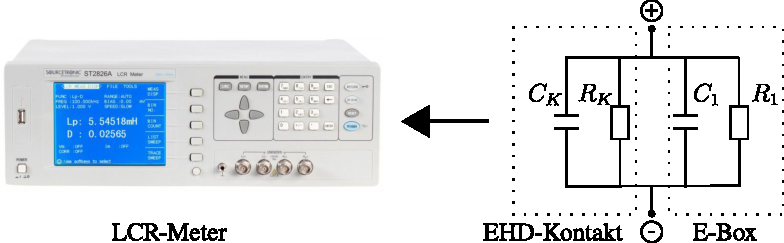
\includegraphics[]{./images/versuchsaufbau_mit_lcr_meter.pdf}
    \caption{Versuchsaufbau zur Kapazitätsmessung mit LCR-Meter}
    \label{fig:versuchsaufbau_zur_kapazitaetsmessung_mit_lcr_meter}
\end{figure}

Das LCR-Messgerät bietet einen breiten Frequenzbereich von \SI{20}{\Hz} bis \SI{50}{\MHz}.
Dank der Kelvin-Messproben (4-Punkt Messung) hat das Gerät eine sehr gute Genauigkeit von \SI{0.1}{\percent} und ermöglicht die Messung auch bei kleinsten Änderung des Systems.
Mit einer Sinuskorrelationstechnik bietet das Gerät eine rauschfreie Analyse.
Die Addition des Widerstands $R_1$ und des Kondensators $C_1$ ist nötig, um zu sehen, ob der Strom tatsächlich durch den EHD-Kontakt fließt oder in irgeneiner Verbindung verloren geht.
Unterschiedliche Werte für $R_1$ und $C_1$ werden verwendet, um deren Einfluß auf die gemessene Kapazität zu untersuchen.
Ein Erhöhung des Widerstandswertes führt zu einer signifikanten Abnahme der Messergebnisse und umgekehrt.
Dieses Phänomen kann durch die Abnahme bzw. Zunahme des Stromflusses durch den EHD-Kontakt erklärt werden.
Die Werte $R_1 = 2$ \si{\kilo\ohm} und $C_1 = 24$ \si{\pico\farad} wurden durch Experimente für die Messungen in dieser Arbeit gewählt.
Abbildung~\ref{fig:lcr_ebox_capacitance} zeigt die Kapazitätsmessung des E-Box (offen) mit dem LCR-Messgerät bei verschiedenen Frequenzen an.

% ----------------------------------------
% Fig: Messprobe mit 24 pF mit dem LCR-Meter
% ----------------------------------------
\begin{figure}[htb]
    \centering
    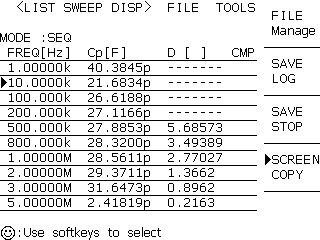
\includegraphics[width=0.5\linewidth]{./images/lcr_ebox_capacitance.jpg}
    \caption{Kapazitätsmessung des E-Box mit dem LCR-Messgerät}
    \label{fig:lcr_ebox_capacitance}
\end{figure}

% ----------------------------------------
% Sec: Versuchsplan
% ----------------------------------------
\section{Versuchsplanung}
\label{sec:versuchsplanung}

Bevor die Messung an dem PCS-Messgerät losgeht, wird zuerst der Zusammenhang zwischen der Filmdicke und der Kapazität im EHD-Kontakt bzw. deren Verhalten unter den Einfluß von der Geschwindigkeit, der Temperatur, der Last und dem Öl theoretisch analysiert.
Anhand dieser Informationen kann man die Testbedingungen, mit den gute Ergebnisse produziert werden, besser auswählen.

Die Schmierfilmdicke kann nach \textit{Hamrock} und \textit{Dowson} (Abschnitt~\ref{sec:schmierfilmdicke_nach_hamrock_und_dowson}) bestimmt werden.
Die Kapazität in dem EHD-Kontakt wird nach dem Modell eines Plattenkondensators (Abschnitt~\ref{sub:kapazitatmessung}) ermittelt.

In Abbildung~\ref{fig:filmdicke_kapazitaet_geschwindigkeit} wird die Schmierfilmdicke und die Kapazität des Öls \textit{SHC320} in Abhängigkeit mit der Geschwindigkeit dargestellt.
Man kann deutlich sehen, während die Filmdicke bei steigender Wälzgeschwindigkeit zunimmt, sinkt die Kapazität in dem Kontakt.
Aus diesem Grund ist die kapazitive Messmethode zur Bestimmung eines dickeren Schmierfilm nicht geeignet.
Bei niedriger Geschwindigkeit hat man besser Auflösung, allerdings besteht es die Gefahr, durch die Berührung von Rauheitsspitzen der Oberfläche der Kugel und der Scheibe das Messergebnis verfälscht wird.
% ----------------------------------------
% Fig: Der Zusammenhang zwischen Filmdicke und Kapazität nach Geschwindigkeit
% ----------------------------------------
\begin{figure}[htb]
    \centering
    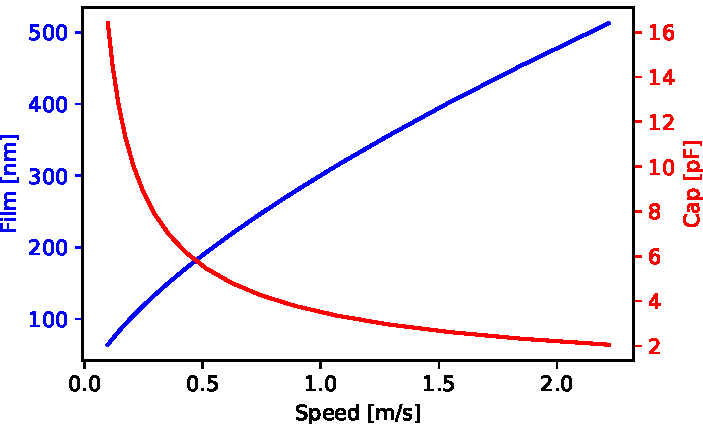
\includegraphics[]{./images/film_cap_speed_80C_20N_SHC320.pdf}
    \caption{Der Zusammenhang zwischen Schmierfilmdicke und Kapazität mit der Geschwindigkeit von dem \textit{SHC320} bei \SI{80}{\degreeCelsius} und \SI{40}{\N}}
    \label{fig:filmdicke_kapazitaet_geschwindigkeit}
\end{figure}

Abbildung~\ref{fig:film_cap_with_dif_temp_and_load} zeigt, dass die Temperatur und die Last relativ große Wirkung auf die Filmdicke und die Kapazität haben.
Bei hohen Temperatur sinkt die Viskosität des Öls ab, was infolge negative Wirkung auf die Filmdicke hat und dadurch wird die Kapazität erhöht.
Analog kann man für steigende Last sagen, allerdings hat die Last zum Vergleich mit der Temperatur wenigeren Einfluß.
% ----------------------------------------
% Fig: Auswirkung der Temperatur auf Filmdicke und Kapazität
% ----------------------------------------
\begin{figure}[htb]
    \centering
    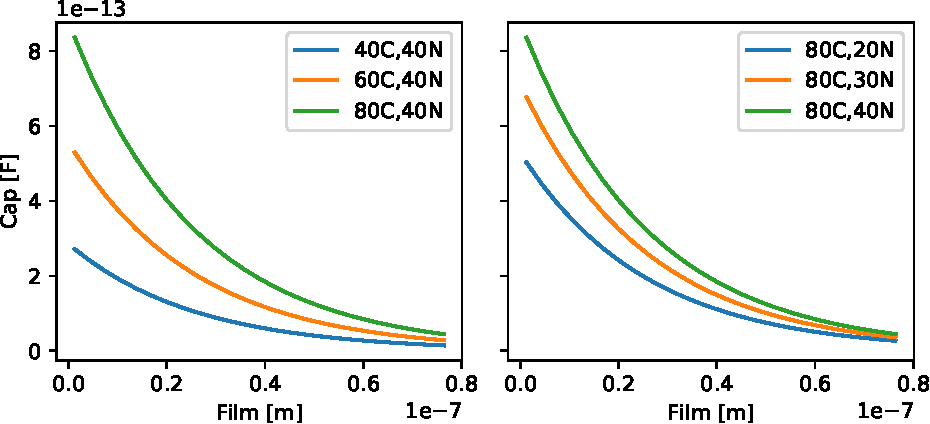
\includegraphics[]{./images/film_cap_with_dif_temp_and_load_fva3.pdf}
    \caption{Zusammenhang zwischen der Kapazität und der Filmdicke bei verschiedenen Temperaturen und Lasten des Öl \textit{FVA3}}
    \label{fig:film_cap_with_dif_temp_and_load}
\end{figure}
\improvement[inline]{fig of cap vs film with dif temp and load}

Die Versuche in dieser Arbeit werden wie folgt geplant und durchgeführt:
% ----------------------------------------
% Enum: Versuchsplan
% ----------------------------------------
\begin{enumerate}
    \item Vergleichsmessungen von neu modifizierten Bauteilen (Kugel, Support, Glasscheibe) mit den von \textit{PCS}
    \item Schmierfilmdickenmessung am EHD-Gerät (optisch)
    \item Schmierfilmdickenmessung mit dem mobilen Messsystem von IMKT (elektrisch)
    \item Vergleich der theoretischen Schmierfilmdickenbestimmung mit 2. und 3. zur Überprüfung des Messverfahrens
\end{enumerate}

% ----------------------------------------
% Sec: Versuchdurchführung
% ----------------------------------------
\section{Versuchdurchführung}
\label{sec:versuchdurchfuehrung}

Da die Auswertung der Schmierfilmdicke in dieser Arbeit optisch und elektrisch geschieht, ist die Sauberkeit vor dem Beginn einer Messung besonders wichtig.
Die Glasscheibe, die Kugel, das Kugelsupport und das Ölreservoir müssen vor jeder Messung mit Waschbenzin oder Isopropanol gereinigt werden und dürfen keine Schlieren aufweisen.

Nach der Reinigung können das Support und die Kugel in das Gerät eingesetzt werden.
Die Führung der Kugel wird zuerst in die Ausgangswelle des zweiten Motors eingesteckt und dann auf das Support aufgelegt.
Die Kabel sollten Abstand von den Wänden des Reservoirs und der Motorwelle halten, um ein Unfall (Kurzschluss der Kugel, Verfangen des Kabels) während des Betriebs zu vermeiden.
Abbildung~\ref{fig:ehd_topf_mit_kugel_und_support} zeigt den Blick von oben auf den EHD-Prüftopf mit montiertem Support und aufgelegter Kugel bereits für den Versuch vorbereitet.

% ----------------------------------------
% Fig: EHD-Prüftopf mit montierten Support und Modifizierter Kugelführung
% ----------------------------------------
\begin{figure}[htb]
    \centering
    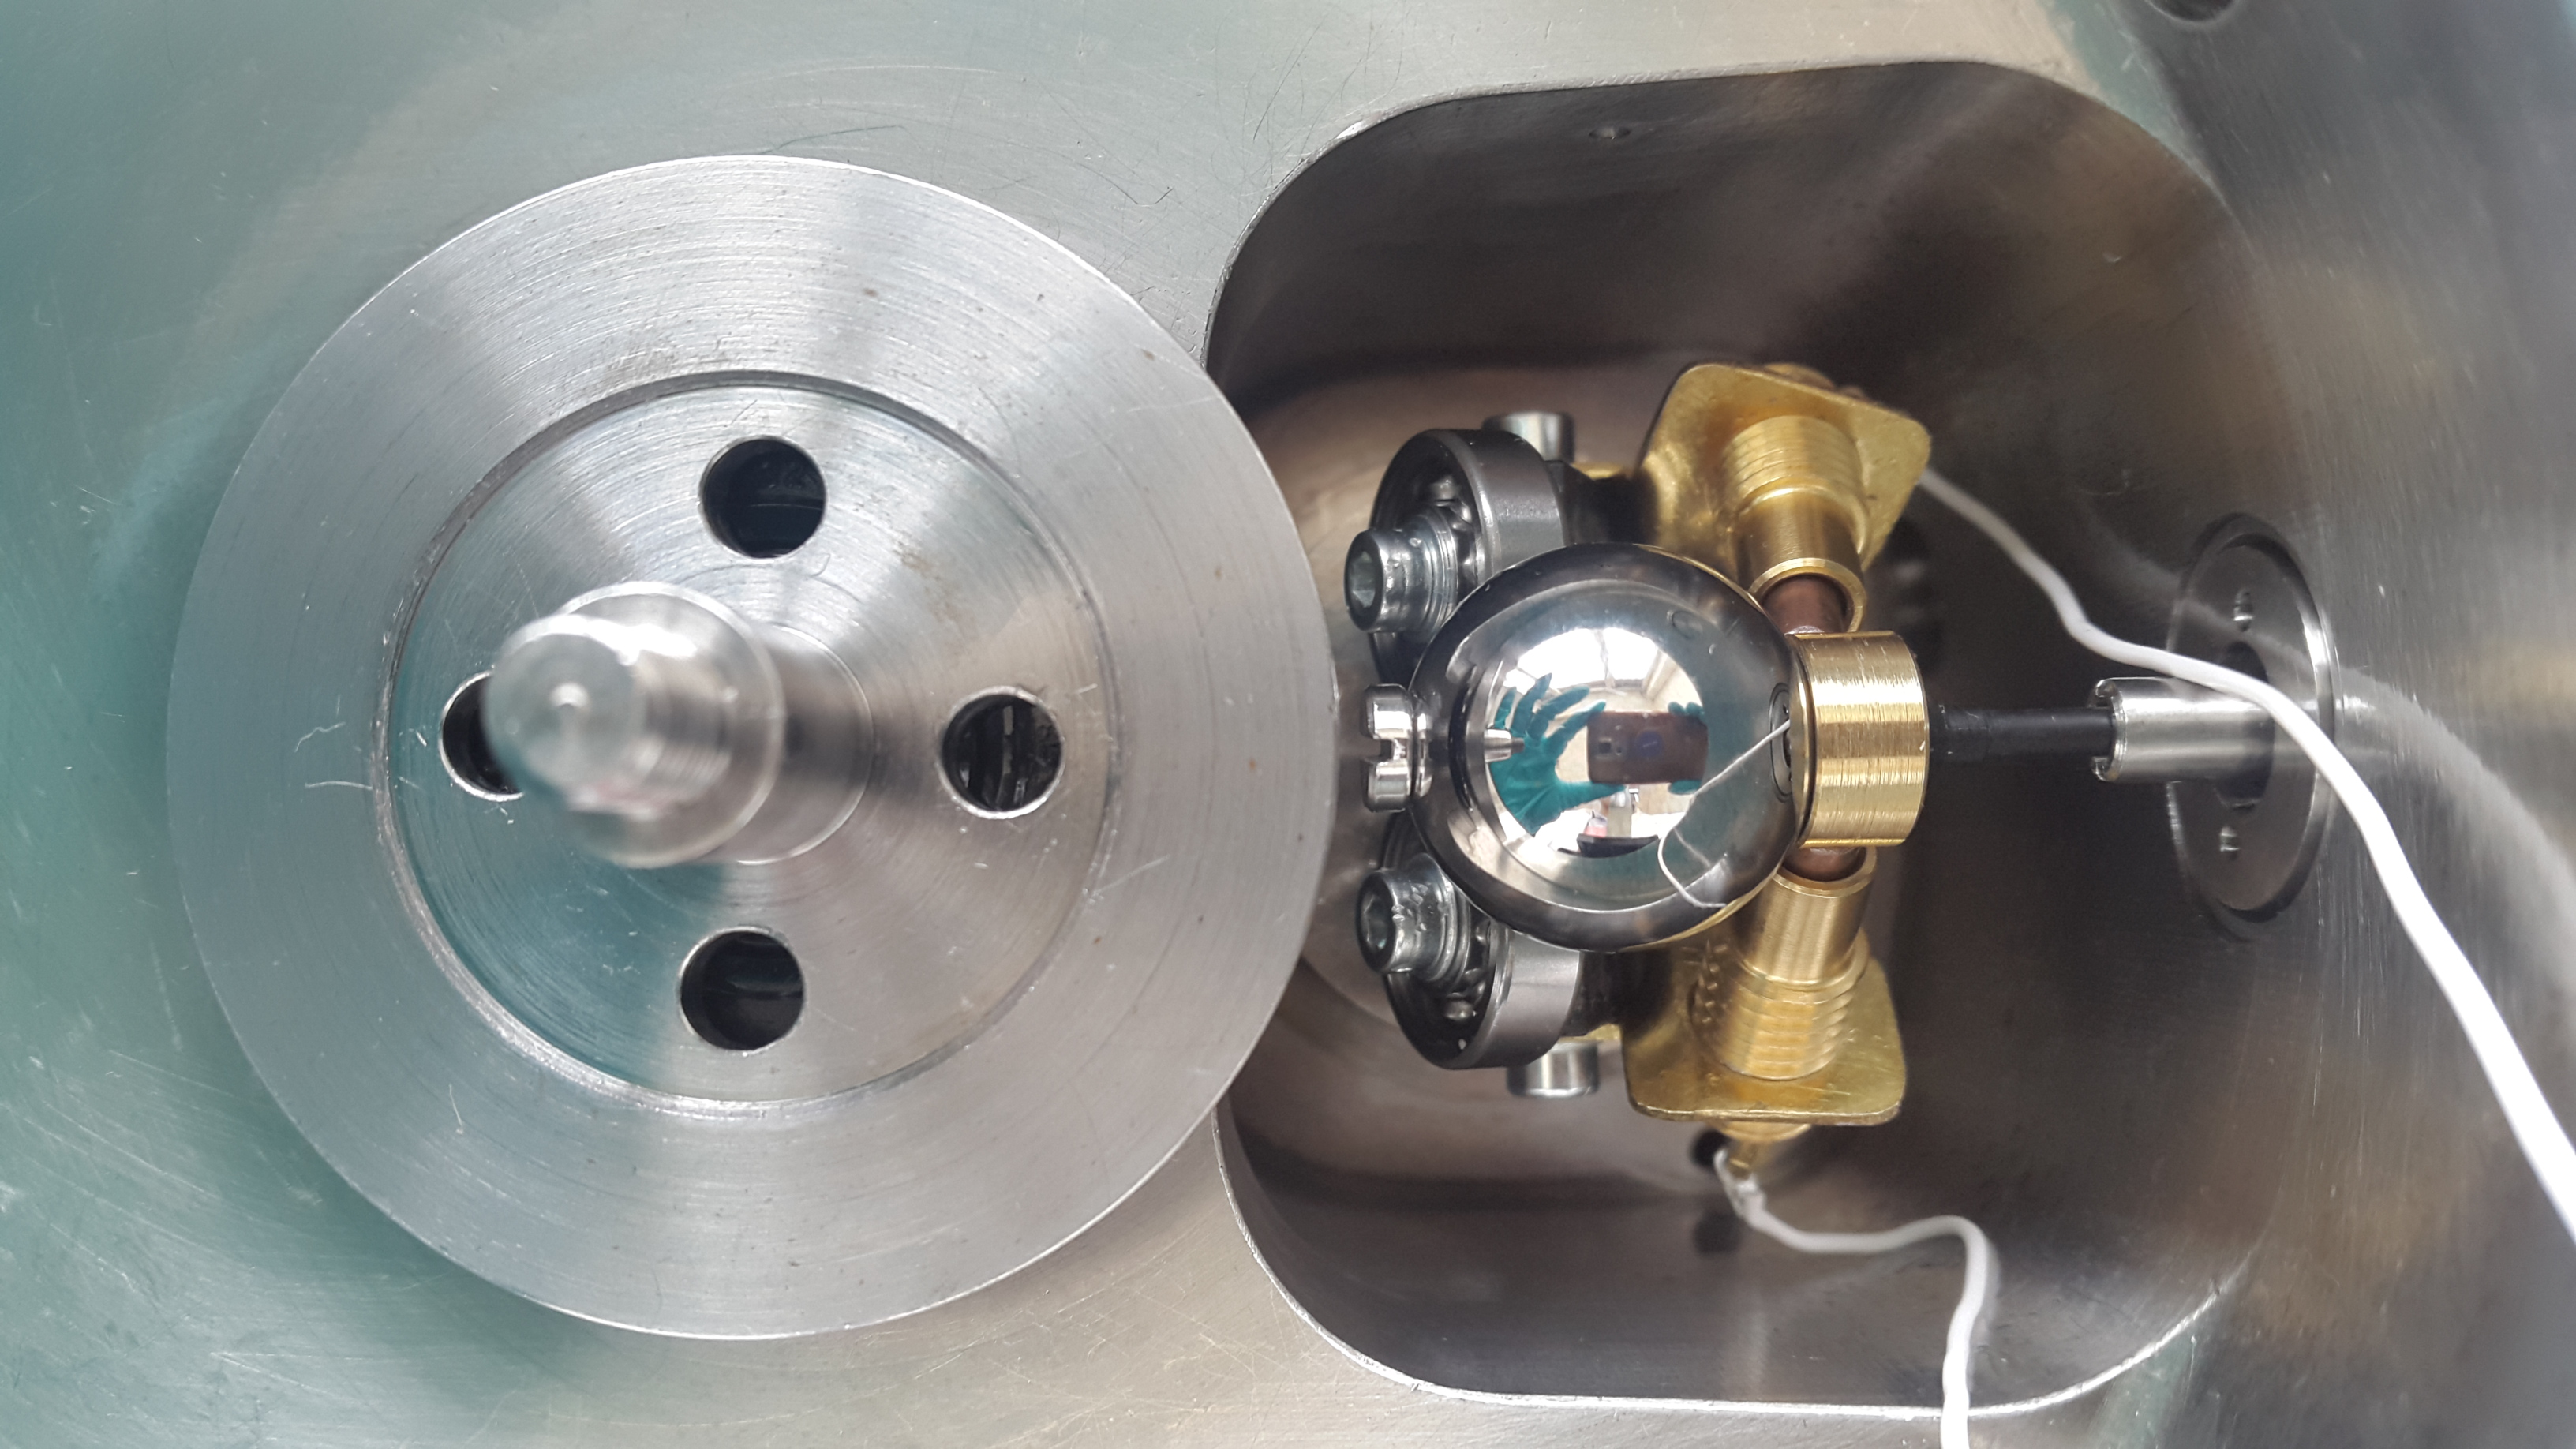
\includegraphics[width=0.7\linewidth]{./images/ehd_topf_mit_kugel_und_support.jpg}
    \caption{Topf des EHD-Geräts mit montiertem neuen Kugelsupport und der modifizierten Kugelführung}
    \label{fig:ehd_topf_mit_kugel_und_support}
\end{figure}

Die Bestimmung des Messpunkts für die optische Messung erfolgt zuerst auf der nicht beschichteten Seite der Scheibe.
Da nach wird die Scheibe um \SI{180}{\degree} auf der Cr-Seite gedreht, um den Widerstand der gesamten Messkette (Kabel -> Scheibe -> Kugel -> Kabel) unter einer Last von \SI{20}{\newton} zu messen.
Der Widerstand ist von dem Radius der Fahrspur abhängig und beträgt ungefähr \SIrange{17}{18}{\ohm}.
Die Suche nach dem Messpunkt findet beim leeren Reservoir statt, weil ein sauberer Kontakt zwischen Scheibe und Kugel für die Bestimmung der Höhe des Spacer-Layers nötig ist.
Außerdem darf man das Spurwechseln nur beim leeren Zustand machen, weil das Verlaufen des Öles über die Lasteinheit im mechanischen Baukasten zu Schäden führen kann.
Man sollte die Spur von außen nach innen wechseln, um die Entstehung von Inseln, die elektronisch zu den Elektroden (Kupferstreifen) isoliert sind, zu vermeiden.
Danach kann man das Öl mit der Hilfe eines Trichters befüllen und den Prüftopf mit dem Deckel schließen.
Abbildung~\ref{fig:suche_nach_ehd_kontakt} zeigt die Suche nach einem guten EHD-Kontakt an.

% ----------------------------------------
% Fig: Bestimmung des Messpunkts
% ----------------------------------------
\begin{figure}[htb]
    \centering
    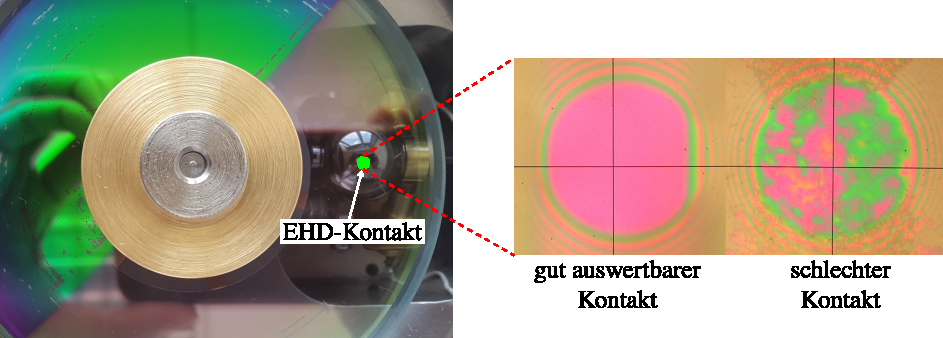
\includegraphics[]{./images/suche_nach_ehd_kontakt.pdf}
    \caption{Die Suche nach einem gut auswertbaren EHD-Kontakt}
    \label{fig:suche_nach_ehd_kontakt}
\end{figure}

Zur Messung bei der Öl-Vollschmierung wird das Ölreservoir bis zur Hälfte der Kugel (ca. \SI{120}{\ml}) gefüllt.
Das Ölbad wird vor jeder Messreihe während des Heizvorgangs (bei \SI{40}{\degreeCelsius}, \SI{60}{\degreeCelsius} und \SI{80}{\degreeCelsius}) für ca. \SI{10}{\minute} durchmischt, damit beim Versuch eine homogene Temperatur im Ölbad herrscht.
Das genaue Vorgehen einer solchen Messung wurde von \textit{Surborg} in seiner Arbeit~\cite{surborg_2007} beschrieben und ist im Anhang zu finden.

Neben dem Widerstand des Kontakts wird auch die Hintergrund-Kapazität des Prüfstands gemessen.
Dieser Wert wird als Störkapazität bezeichnet und soll von der Ergebnissen abgezogen werden.

Die Last von \SI{20}{\newton} wird in Anlehnung an vorherige Arbeiten gewählt.
Nach dem Abschnitt~\ref{sec:betrachtung_des_ehd_kontaktes} lässt sich für den hier betrachteten Fall eines Kugel-Scheibe-Modells eine maximale Pressung im Kontakt $p_0 =$ \SI{509}{\mega\pascal} berechnen.
Damit liegt der Kontakt im unteren Bereich der EHD-Schmierung.
Diese geringe Last ist gut, somit wird die Gefahr von Beschädigungen auf der Scheibe bzw. der Silikatschicht gering gehalten.

Nachdem die Höhe des Spacer-Layers bestimmt wurde, wird die Scheibe ein Stück weiter gedreht und auf etwa \SI[per-mode=symbol]{100}{\mm\per\second} beschleunigt.
Während dieser Einlaufphase wird das Live Bild ständig auf dem SW-Monitor beobachtet.
Sobald sich ein klarer, gut messbarer Verlauf abzeichnet, kann man mit der Messung begonnen werden (siehe Abbildung~\ref{fig:ehd_live_bild}).
Wichtig ist, dass man die Messungen zügig macht, um die Beschädigung der Chromschicht und Silikatschicht zu vermeiden.

% ----------------------------------------
% Fig: Schlechtes und gutes Live Bild
% ----------------------------------------
\begin{figure}[htb]
    \centering
    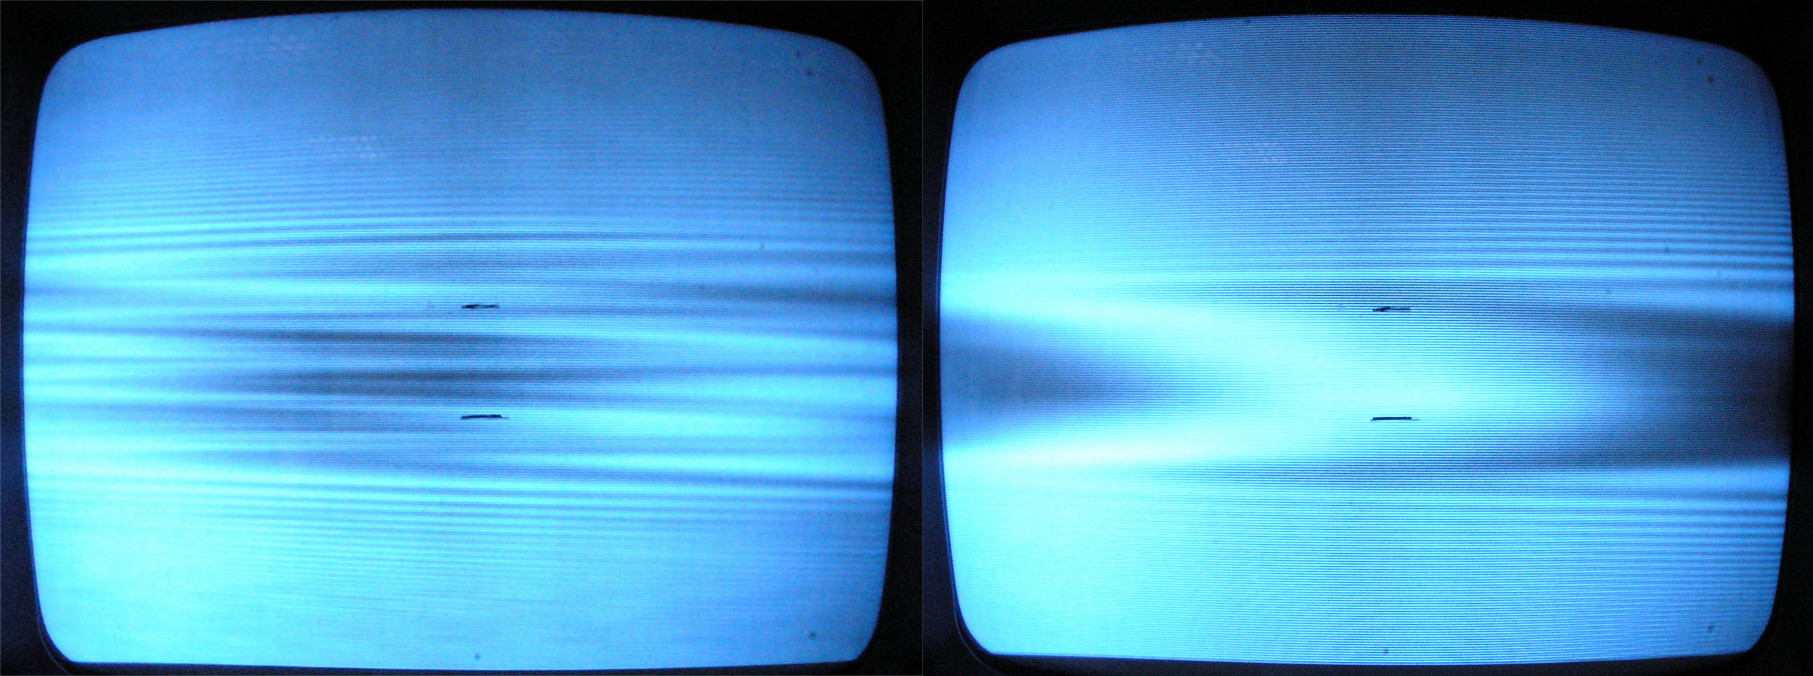
\includegraphics[width=0.8\linewidth]{./images/ehd_live_bild.jpg}
    \caption{Live Bild: nicht verwertbarer Verlauf (links); guter Verlauf (rechts)~\cite{mach_2008}}
    \label{fig:ehd_live_bild}
\end{figure}

Tabelle~\ref{tab:ehd_test_params} und~\ref{tab:einstellungen_des_ladekurve_messsystems} fassen die Versuchsparameter und die Einstellungen für das mobile Messsysten von IMKT zur Schmierfilmdickemessung in dieser Arbeit zu.

% ----------------------------------------
% Tab: Versuchsparameters am EHD-Prüfstand
% ----------------------------------------
\begin{table}[htbp]
    \centering
    \caption{Versuchsparameters beim EHD-Prüfstand}
    \begin{tabular}{ll}
        Öl & FVA 3 \\
        Last [\si{N}] & 20 \\
        Temperatur [\si{\degreeCelsius}] & 40 – 60 – 80 \\
        Geschwindigkeit [\si[per-mode=symbol]{\meter\per\second}] & \SIrange[per-mode=symbol]{0.1}{1.4}{\meter\per\second} \\
        Geschw. Stufen [\si{\%}] & 40 \\
        Schlupf [\si{\%}] & 0; 5 \\
    \end{tabular}
    \label{tab:ehd_test_params}
\end{table}


% ----------------------------------------
% Tab: Einstellungen des mobilen Messsystems von IMKT
% ----------------------------------------
\begin{table}[htbp]
    \centering
    \caption{Einstellungen des mobilen Messsystems von IMKT}
    \begin{tabular}{ll}
        Messtyp                          & Anzahl der Messwerte \\
        Anzahl der Messwerte [\si{1}]    & 2500                 \\
        Anzahl der Ladekurven [\si{1}]   & 10                   \\
        Abtastrate [\si{\Hz}]            & 250000               \\
        Ladespannung [\si{\volt}]        & 0.2                  \\
        Verzögerung [\si{\ms}]           & 1                    \\
        Entladezeit [\si{\ms}]           & 100                  \\
        Ladevorwiderstand [\si{\ohm}]    & 1012700              \\
        Störkapazität [\si{\pico\farad}] & 0                    \\
    \end{tabular}
    \label{tab:einstellungen_des_ladekurve_messsystems}
\end{table}



